\documentclass[twocolumn]{jarticle}
\usepackage[dvipdfmx]{graphicx}
\usepackage{appi2013_2}

%%packages related to equations and math letters
\usepackage{amsmath,amssymb,amsfonts}
\usepackage{amsthm} %定理環境.
%\usepackage{theorem} %定理環境.amsthmを使う場合はコメントアウト.
\usepackage{siunitx} %単位,数値に必要.
\usepackage{latexsym}
\usepackage{empheq} %連立方程式に用いる
%\usepackage{array} %連立方程式に用いる.empheq環境でよい.
%%

%packages related to fonts
\usepackage{bm}
\usepackage{bbm}
\usepackage{otf}
\usepackage[dvipdfmx]{color}
\usepackage[version=3]{mhchem} %化学式を出力するときに用いる.
%\usepackage{newtxtext,newtxmath} %Times フォント関係のパッケージ.
\usepackage{times} % TimesとHelveticaを使う。数式はComputer Modern
%%

%%packages related to structure of the text
\usepackage{ascmac} %make frames
\usepackage{enumerate} %make lists
%\usepackage{enumitem} %customize package of enumerate
%%
%%packages related to quote
%\usepackage{cite}
\usepackage{url}
\usepackage[superscript]{cite}  %参考文献番号を上付にしないなら要らない
\renewcommand\citeform[1]{[#1]} %cite.styを使わないときにはこれもコメントにすること
%%

%%packages related to algorithm and source code
\usepackage{algorithm}
\usepackage{algorithmic}
%\usepackage{listings}
%%

%%packages related to figures and tables
\usepackage{wrapfig}
\usepackage{subcaption}
\usepackage{here}
%\usepackage{multirow}
%\usepackage{slashbox}
%\usepackage{longtable}
%\usepackage{float} %here環境と同じ.使う必要はない.
%%
%%package related to comment
\usepackage{comment} %\begin{comment} ~ \end{comment}でコメントアウトできる.
%%
%%package related to pdf
\usepackage{pdfpages}

\usepackage{mathtools}
\usepackage[labelformat=parens, justification=raggedright]{subcaption}
\newcommand{\rfig}[1]{Fig.~\ref{#1}}
\newcommand{\req}[1]{式\eqref{#1}}


\jtitle{\fontsize{13pt}{0pt}相互通信可能な分子通信系シミュレーションによる濃度依存性の検証}
\etitle{Two-step reinforcement learning for model-free redesign of nonlinear optimal regulator}
\lab{堀}
\no{82411805}
\name{川口竜輝}
\begin{document}
\maketitle

\section{研究背景・目的}
自然界において,細胞はシグナル分子と呼ばれる伝達物質を別の細胞に送ることで
情報の伝達を行っている.このような細胞間の情報伝達を相互に行う系は分子通信系と呼ばれ,
系は細胞内での化学反応と細胞間のシグナル分子の伝達によって構成されている.
分子通信系では,系内部の細胞の濃度が系全体の状態に影響を与えることが知られているが,
その量的な関係を調べた研究は少ない.


\section{相互通信可能な分子通信系}
状態$\bm{x}_{k} \in \mathbb{R}^{n}$,入力$\bm{u}_{k} \in \mathbb{R}^{m}$に関するコスト関数
\begin{align}
    \sum^{\infty}_{k=0} \gamma^{k} (\bm{x}_{k}^\top Q \bm{x}_{k} + \bm{u}_{k}^\top R \bm{u}_{k})
    \label{eq:cost_equation}
\end{align}
を最小にするような制御器を設計する問題を考える.ただし,$Q \in \mathbb{R}^{n \times n}, R \in \mathbb{R}^{m \times m}$はそれぞれ半正定値,正定値行列であり,$\gamma \in (0, 1)$は
%割引率と呼ばれる
定数である.
この問題に対し,\rfig{fig:proposed_method}で表される制御器の設計を2つのステップに分けて行う.

Step~1ではまず,既知の安定なフィードバックゲイン$K^{\mathrm{init}}$を用い,探索項を印加しながらシステムを動かすことで入力と状態の時系列データを取得する.
その後,ベルマン方程式から導出される関係式
\begin{align}
F ^j [\textrm{vec}(G^{j+1}_1)^\top ,\textrm{vec}(G^{j+1}_2)^\top ,\textrm{vec}(G^{j+1}_3)^\top]^\top=\bm{h}^j
\label{update_equation}
\end{align}
によって$G^{j+1}_i,~i=1,2,3$
を更新し,
$K^{j+1}=-(R+G_3^{j+1})^{-1}G_2^{j+1}$
% \begin{align}
%     K^{j+1}=-(R+G_3^{j+1})^{-1}G_2^{j+1}
% \end{align}
に代入することで
%フィードバックゲイン
$K^j$の更新を行う.
ただし,$\bm{h}^{j}$は各時刻における
二次コストに関するベクトル,
$F^{j}$は入力と状態に関する行列,
$G^{j+1}_i$は
コスト関数に関する行列であり,
$F^j,~ \bm{h}^j$は取得した時系列データと$K^j$から計算される.
$||K^j-K^{j-1}||$が閾値以下になったら更新を終了し,このときの$K^j$を$K^{\rm{AC}}$とする.更新される$K^{j}$は,準最適線形LQR制御則に収束する.

Step~2では,Step~1で設計された線形制御器と並列に繋げた非線形制御則$\bm{\mu}$を強化学習の一種であるActor-Critic法\cite{Sutton_RL}によって設計する.
線形制御則$K^{\rm{AC}}$が存在することで,学習中にシステムが不安定になることを防ぎ,損耗を防ぐことができる.
この二段階の設計手法による制御則は,線形制御則だけでは実現できない性能を達成する.

\begin{figure}[tb]
    \centering
    \includegraphics[width=\columnwidth] {figures/model_free_two_step_controller_design_characterless.pdf}
    \caption{Structure of the proposed method}
    \label{fig:proposed_method}
\end{figure}


\section{数値例による検証}
数値シミュレーションを用いて,次のような相互通信可能な1次元分子通信系を考える.
Fig. にあるように,1次元分子通信系において細胞が2つ存在し,
数値シミュレーションを用いて,提案法 ($K^{\mathrm{AC}}$ + RL) ,$K^{\mathrm{init}}$と強化学習を組み合わせた方法($K^{\mathrm{init}}$ + RL),強化学習単独(RL alone) ,補助制御器単独 ($K^{\mathrm{AC}}$ alone) の4つの場合について,倒立振子の制御器設計を行った.
Step 2における各試行ごとの二次コストを\rfig{fig:simulation}に示す.
\rfig{fig:simulation}より,提案法は他の方法と比べて,学習初期のコストが小さく,過渡学習性能が良いことが示された.
\begin{figure}[tb]
    \centering
    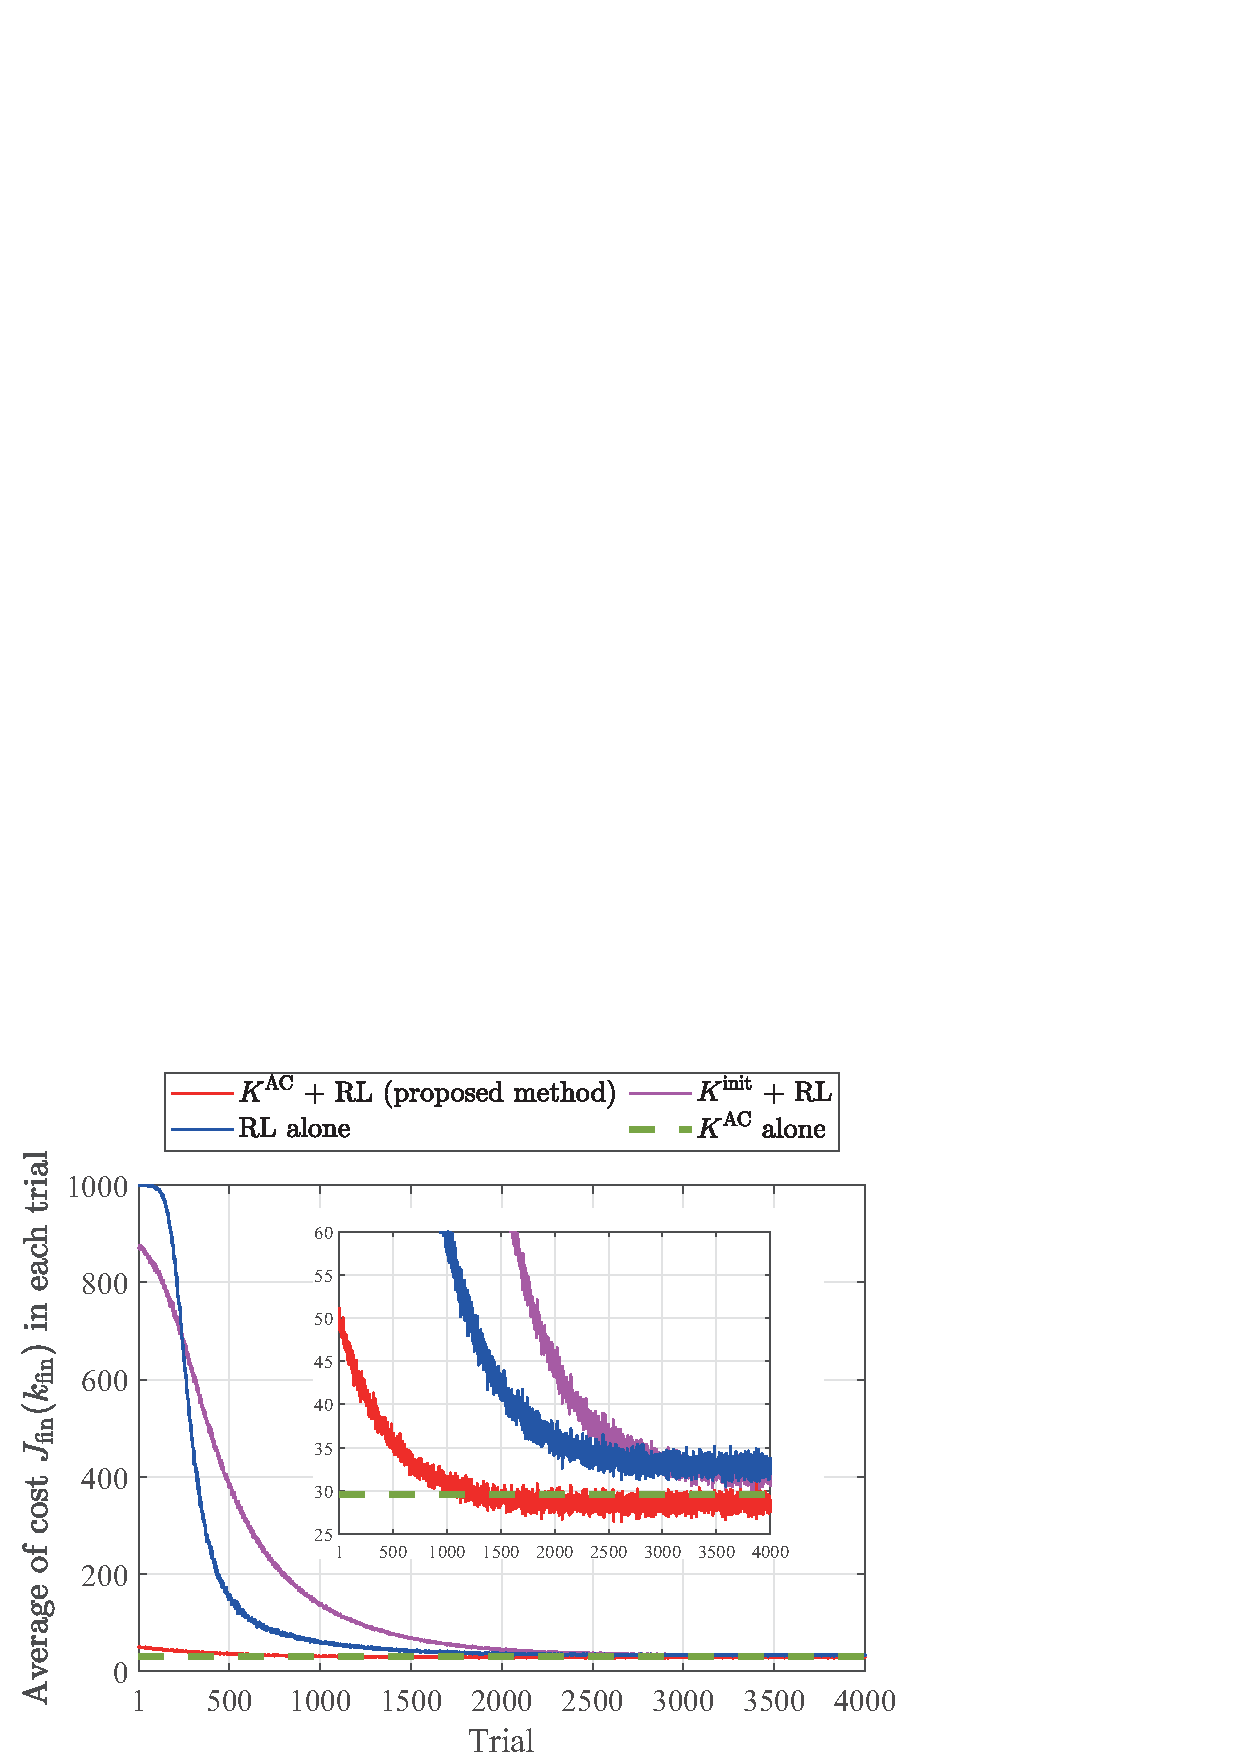
\includegraphics[width=\columnwidth]{figures/step2_cost_fig.pdf}
    \caption{Cost $J_\mathrm{fin}(k_{\mathrm{fin}})$ in each trial in Step~2. Inset is plotted with in a different scale of the vertical access. %to high-light the average cost at the end the learning process.
    }
    \label{fig:simulation}
\end{figure}


\section{結論と今後の展望}
本稿では,密度依存的な分子通信系のシミュレーション法構築に向けて,
相互通信可能な1次元の分子通信系の数値シミュレーションを行った.
具体的には,細胞内でシグナル分子が作成



\begin{thebibliography} {99}
    \bibitem{Sutton_RL} R. S. Sutton {\it et al}., %Reinforcement learning: An introduction,
    2nd ed. { \it MIT Press}, 2018.
    \bibitem{Kiumarsi2018} B. Kiumarsi {\it et al}., 
    %“Opti-mal and autonomous control using reinforcement learning: A survey, ”
    {\it IEEE Transactions on Neural Networks and Learning Systems}, vol. 29, no. 6, pp. 2042–2062, 2018.
\end{thebibliography}

\end{document}
